% ============================================================
% Project Management Plan — LaTeX Template
% Converted from Project Management Plan Template.docx
% Compile with: pdflatex (twice for TOC)
% ============================================================
\documentclass[12pt,a4paper]{article}

% ---- Encoding & fonts ----
\usepackage[T1]{fontenc}
\usepackage[utf8]{inputenc}
\usepackage{lmodern}
\usepackage{microtype}

% ---- Page layout ----
\usepackage[left=2.54cm,right=2.54cm,top=2.54cm,bottom=2.54cm,
            headheight=1.5cm]{geometry}

% ---- Colors ----
\usepackage{xcolor}
\definecolor{heading}{RGB}{68,84,106}       % #44546A dark blue-grey
\definecolor{accent}{RGB}{91,155,213}       % #5B9BD5 light blue
\definecolor{instrcolor}{RGB}{127,127,127}  % grey for instruction text
\definecolor{tabheadbg}{RGB}{68,84,106}     % table header background
\definecolor{tabheadfg}{RGB}{255,255,255}   % table header text (white)
\definecolor{rowalt}{RGB}{220,230,242}      % alternate row shading

% ---- Graphics & tables ----
\usepackage{graphicx}
\usepackage{tabularx}
\usepackage{booktabs}
\usepackage{array}
\usepackage{colortbl}
\usepackage{longtable}
\usepackage{multirow}
\newcolumntype{L}[1]{>{\raggedright\hbadness=10000\hfuzz=15pt\arraybackslash}p{#1}}
\newcolumntype{C}[1]{>{\centering\arraybackslash}p{#1}}

% ---- Section headings ----
\usepackage{titlesec}
\titleformat{\section}[hang]
  {\Large\bfseries\color{heading}}{\thesection}{1em}{}
  [\vspace{-0.3em}\color{accent}\rule{\linewidth}{0.8pt}\vspace{0.3em}]
\titleformat{\subsection}[hang]
  {\large\bfseries\color{heading}}{\thesubsection}{1em}{}
\titleformat{\subsubsection}[hang]
  {\normalsize\bfseries\color{heading}}{\thesubsubsection}{1em}{}
\titlespacing*{\section}{0pt}{1.5ex plus .5ex minus .2ex}{0.8ex}
\titlespacing*{\subsection}{0pt}{1.2ex plus .4ex minus .2ex}{0.6ex}
\titlespacing*{\subsubsection}{0pt}{1ex plus .3ex minus .2ex}{0.4ex}

% ---- Header / Footer ----
\usepackage{fancyhdr}
\pagestyle{fancy}
\fancyhf{}
\lhead{\small\color{heading}\textit{PROJECT MANAGEMENT PLAN}}
\rhead{
\includegraphics[height=0.75cm]{figures/pmp_header.png}}
\cfoot{\small\thepage}
\renewcommand{\headrulewidth}{0pt}

% ---- TOC & Hyperlinks ----
\usepackage[bookmarks,colorlinks,
            linkcolor=heading,urlcolor=accent,
            pdftitle={Project Management Plan}]{hyperref}

% ---- Paragraph spacing ----
\usepackage{parskip}
\setlength{\parskip}{5pt}
\setlength{\parindent}{0pt}

% ---- Enumeration ----
\usepackage{enumitem}
\setlist[itemize]{nosep,topsep=2pt}

% ---- Helper commands ----
% Instruction placeholder (grey italic, shown in angle brackets)
\newcommand{\instr}[1]{%
  \textcolor{instrcolor}{\textit{\textless{}#1\textgreater{}}}}

% Table header row macro
\newcommand{\thead}[1]{%
  \cellcolor{tabheadbg}\textcolor{tabheadfg}{\textbf{#1}}}

% ============================================================
\begin{document}

% ============================================================
%  TITLE PAGE
% ============================================================
\begin{titlepage}
  \thispagestyle{empty}
  \centering

  
\includegraphics[width=\textwidth]{figures/pmp_header.png}\\[1.5cm]

  {\fontsize{28}{34}\selectfont\bfseries\color{heading}
    PROJECT MANAGEMENT PLAN\\[0.8cm]}

  {\Large\color{heading}\instr{Project Name}\\[0.4cm]}

  {\large Group \instr{Group Number}\\[0.4cm]}

  {\normalsize\instr{Author Names}\\[1.5cm]}

  {\large\bfseries\color{heading} Planning Phase\\[0.3cm]}

  {\normalsize\today}

  \vfill
\end{titlepage}

% ============================================================
%  DOCUMENT INSTRUCTIONS (remove when complete)
% ============================================================
\thispagestyle{empty}
\begin{center}
  {\large\bfseries\color{heading} Using This Template}
\end{center}

\noindent
\colorbox{rowalt}{\parbox{\dimexpr\linewidth-2\fboxsep}{%
\small
To create a Project Management Plan from this template:
\begin{itemize}
  \item Replace \texttt{\textless{}...\textgreater{}} placeholders throughout with
        project-specific content.
  \item Remove or delete all grey instruction paragraphs once the
        relevant section is complete.
  \item Update the Table of Contents by recompiling the document twice
        with \texttt{pdflatex}.
  \item Delete this instruction page when the plan is finalised.
\end{itemize}
}}

\vspace{1em}
\begin{center}
  {\bfseries Document Purpose}
\end{center}
The Project Management Plan defines the project objective and scope as
well as how it is executed, monitored, and controlled during the
Delivery Stage.

\vspace{0.5em}
\noindent{\bfseries Who Produces This Document}\\
The assigned Project Manager produces the Project Management Plan in
collaboration with the project team members and in consultation with
the functional organizations involved in the managerial and technical
processes described herein.

\clearpage

% ============================================================
%  REVISION HISTORY
% ============================================================
\thispagestyle{fancy}
\begin{center}
  {\Large\bfseries\color{heading} Revision History}
\end{center}

\vspace{0.5em}
\noindent
\begin{tabularx}{\linewidth}{C{2cm}|X|C{3cm}|C{3cm}}
  \thead{Version} & \thead{Description} & \thead{Date Modified} & \thead{Author}\\
  \hline
  1.0 & & & \\[4pt]
  \hline
      & & & \\[4pt]
  \hline
      & & & \\[4pt]
  \hline
      & & & \\[4pt]
  \hline
      & & & \\[4pt]
  \hline
      & & & \\[4pt]
\end{tabularx}

\vspace{1.5em}
\begin{center}
  {\Large\bfseries\color{heading} Authority Signatures}
\end{center}

\vspace{0.3em}
\noindent The Project Lead (Business Side) and the Project Manager agree to
deliver the Delivery Stage of this project in accordance with this
Project Management Plan and amend it periodically as project parameters
change.

\vspace{0.8em}
\noindent{\bfseries Prepared by:}\\[0.5em]
\begin{tabularx}{\linewidth}{|X|X|X|X|}
  \hline
  \thead{Prepared by:} & \thead{Prepared by:} & \thead{Prepared by:} & \thead{Prepared by:}\\
  \hline
       & & & \\[6pt]
  \hline
       & Signature & Signature & Signature \\[6pt]
  \hline
  Please print: & Please print: & & \\[4pt]
  \hline
       & Name & ID & Date \\[4pt]
  \hline
\end{tabularx}

\vspace{0.8em}
\noindent{\bfseries Approved by:}\\[0.5em]
\begin{tabularx}{\linewidth}{|X|X|X|X|}
  \hline
  \thead{Approved by:} & \thead{Approved by:} & \thead{Approved by:} & \thead{Approved by:}\\
  \hline
       & & Signature & Signature \\[6pt]
  \hline
       & & & \\[6pt]
  \hline
  Please print: & & & \\[4pt]
  \hline
       & Name & Title & Date \\[4pt]
  \hline
\end{tabularx}

\clearpage

% ============================================================
%  TABLE OF CONTENTS
% ============================================================
\tableofcontents
\clearpage

% ============================================================
%  SECTION 1: EXECUTIVE SUMMARY
% ============================================================
\section{Executive Summary}

\instr{Describe the key issues driving the project. Clearly demonstrate
the problem/opportunity and how resolution of this problem/opportunity
provides best value, while meeting investment plan, business, technical
or legal/political/regulatory objectives. Summarize the results of the
Project Identification Stage (e.g.\ feasibility assessment and business
case). Define the objectives of the project and the intended results.
Define quantitative and measurable objectives that can be used as
criteria by which key stakeholders will judge the success of the
project. Some of this information can be extracted from the Project
Charter.}

% ============================================================
%  SECTION 2: INTEGRATION MANAGEMENT
% ============================================================
\section{Integration Management}

Integration Management includes all of the processes required to
unify, coordinate and manage all project elements to completion.
Integration Management crosses all phases of projects and includes
change management, execution, control and close out. Briefly describe
how this will be accomplished.

% --- 2.1 ---
\subsection{Project Team Structure}

\instr{Describe the organizational boundaries between the project and
external entities. Define and describe communication with senior
management, customers, subcontractors, purchasing, sales, marketing,
legal, finance, procurement, installation and support organizations,
standards or certification bodies, auditors, manufacturing, and the
like.}

\instr{Using a diagram, illustrate corporate governance bodies that may be
involved in the approval process and describe their roles and
responsibilities in Section~\ref{sec:roles}. Illustrate the project
team structure and relationships in a style adapted to the project size
and complexity.}

\vspace{0.5em}
% Org-chart figure — replace path below with your PNG file
\begin{figure}[h]
  \centering
  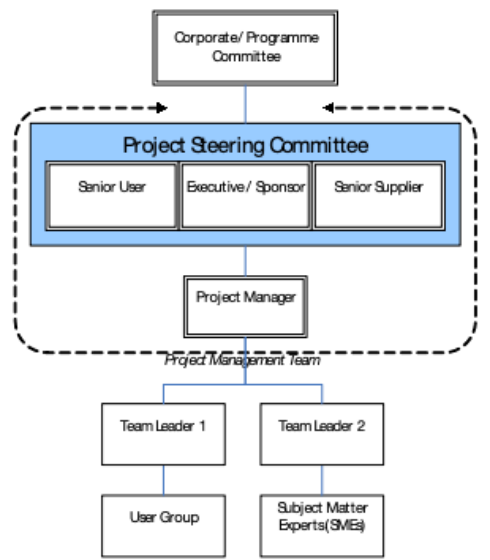
\includegraphics[width=0.7\textwidth]{figures/project_team_structure.png}
  \caption{Project Team Structure}
  \label{fig:orgchart}
\end{figure}

% --- 2.2 ---
\subsection{Roles and Responsibilities}
\label{sec:roles}

\instr{List the major roles identified in the project team structure
diagram as well as internal and external project stakeholders who are
not specifically members of the project team. Describe their relevance
to the project and their degree of interaction for specific project
activities.}

\vspace{0.5em}
\noindent
\begin{tabularx}{\linewidth}{|L{3.5cm}|L{3cm}|X|L{2.5cm}|}
  \hline
  \thead{Project Position} & \thead{Name} & \thead{Responsibilities} & \thead{External Resource}\\
  \hline
  & & & \\[8pt]
  \hline
  & & & \\[8pt]
  \hline
  & & & \\[8pt]
  \hline
  & & & \\[8pt]
  \hline
  & & & \\[8pt]
  \hline
\end{tabularx}

% --- 2.3 ---
\subsection{Change Management}

\instr{Describe how change will be managed throughout the Delivery
Stage of this project. This should include Change Management processes,
roles and responsibilities, tools and techniques and reporting.}

\subsubsection{Change Control}

\instr{Describe the Change Control process that will be used
including:}
\begin{itemize}
  \item Change governance
  \item Change identification and request management
  \item Impact analysis
  \item Change approval process
  \item Change tracking
\end{itemize}

% --- 2.4 ---
\subsection{Project Close Out}

\instr{Include the plans necessary to ensure orderly close out of the
project. Items in the close out plan should include a staff
reassignment plan, a plan for archiving project materials, a plan for
post-mortem debriefings of project personnel, and preparation of a
final report to include lessons learned and analysis of project
objectives achieved.}

% ============================================================
%  SECTION 3: SCOPE MANAGEMENT
% ============================================================
\section{Scope Management}

\instr{Describe how scope will be managed throughout the Delivery Stage
of this project. This could include information on specific Scope
Management processes such as scope verification and control,
development of work breakdown structure, roles and responsibilities,
tools and techniques and reporting.}

% --- 3.1 ---
\subsection{Scope Statement}

\instr{Provide a scope statement, including what is within and what is
not within scope; that is, the scope of the project needed to meet the
stated objective. It is important to keep in mind that scope includes
the requirements for both the product scope (the features and functions
of a product or service) and project scope (the work required to
deliver the product).}

\vspace{0.5em}
\noindent
\begin{tabularx}{\linewidth}{|X|X|}
  \hline
  \thead{Activities In Scope} & \thead{Activities Out of Scope}\\
  \hline
  & \\[30pt]
  \hline
  & \\[30pt]
  \hline
\end{tabularx}

% --- 3.2 ---
\subsection{Requirements Management}

\instr{Requirements will feed into the details of the project and
product scope. Describe how requirements will be gathered, detailed,
validated, controlled and managed. Also include tools and processes
that will be used, such as requirements mapping.}

% --- 3.3 ---
\subsection{Project Deliverables}

\instr{List the major items to be delivered to the customers,
subcontractors, integrators, or other parties. As appropriate, list
the deliverables, their recipients, interim and final delivery dates,
and delivery method.}

\instr{The list should differentiate the project management deliverables
(e.g.\ project schedule, communication plan, progress report, etc.)
from the project deliverables (e.g.\ system, database,
telecommunication equipment, system and user documentation, etc.).}

\vspace{0.5em}
\noindent
\begin{tabularx}{\linewidth}{|X|X|C{2.5cm}|L{3cm}|}
  \hline
  \thead{Deliverable} & \thead{Recipients} & \thead{Delivery Date} & \thead{Delivery Method}\\
  \hline
  & & & \\[8pt]
  \hline
  & & & \\[8pt]
  \hline
  & & & \\[8pt]
  \hline
\end{tabularx}

\subsubsection{Work Activities}

\instr{Specify the various work activities to be performed in the
project. A Work Breakdown Structure should be used to depict the work
activities and the relationships among work activities.}

\subsubsection{Constraints}

\instr{Constraints or restrictions limit or place conditions on the
project, especially those associated with the project scope (e.g.\ a
hard deadline, a predetermined budget, a set milestone, contract
provisions, privacy or security considerations, etc.)}

\subsubsection{Assumptions}

\instr{Assumptions are factors that for planning purposes are
considered to be true, real or certain. These assumptions will be
validated during the planning process in the Delivery Stage.}

\subsubsection{Stakeholders}

\instr{Identify the individuals or organizations (e.g.\ customer,
sponsor, performing organization or the public) that are actively
involved in the project, or whose interests may be positively or
negatively affected by execution or completion of the project.
(PMBOK\textsuperscript{\textregistered}) This is a preliminary
estimate.}

% ============================================================
%  SECTION 4: SCHEDULE MANAGEMENT
% ============================================================
\section{Schedule Management}

\instr{Describe how time will be managed throughout the Delivery Stage
of this project. This should include processes that will be used to
develop the schedule, roles and responsibilities, tools and techniques
and reporting (PDM, CPM).}

% --- 4.1 ---
\subsection{Milestones}

\instr{Identify the significant milestones in the project (phases,
stages, decision gates, approval of a deliverable, etc.). This can
also represent a high-level project schedule.}

\vspace{0.5em}
\noindent
\begin{tabularx}{\linewidth}{|X|C{3cm}|L{3.5cm}|}
  \hline
  \thead{Description} & \thead{Forecast Date} & \thead{Gate / Approval}\\
  \hline
  & & \\[8pt]
  \hline
  & & \\[8pt]
  \hline
  & & \\[8pt]
  \hline
  & & \\[8pt]
  \hline
\end{tabularx}

% --- 4.2 ---
\subsection{Schedule Control}

\instr{Specify the control mechanisms that will be used to measure the
progress of the work completed at milestones. Specify the methods and
tools used to compare actual schedule performance to planned
performance and to implement corrective action when actual performance
deviates from planned or required performance. A project schedule in
the form of a Gantt chart should be created, preferably in a project
tracking tool. Describe how and when schedules will be modified and how
agreement and commitment to the revised schedules will be achieved.}

% ============================================================
%  SECTION 5: COST MANAGEMENT
% ============================================================
\section{Cost Management}

\instr{Describe how cost will be managed throughout the Delivery Stage
of this project. This should include processes that will be used to
develop the budget, roles and responsibilities, tools and techniques
and reporting.}

% --- 5.1 ---
\subsection{Estimation}

\instr{Describes how project estimates will be prepared, including:}
\begin{itemize}
  \item The methods, tools, and techniques that will be used to estimate
        project size, effort, cost, schedule, and critical computer
        resource requirements.
  \item The timing of the estimates.
  \item Who will participate in the estimation process.
  \item How the estimates will be documented, reviewed, and reported.
\end{itemize}
\noindent\instr{You can include the actual estimates in this section or they
can be stored elsewhere. For each estimate made, document the
estimation method used, the assumptions made, and the confidence level
for the estimate. Describe the rationale behind contingency buffers
incorporated into estimates. Specify the methods to be used
periodically to re-estimate the cost, time, and resources needed to
complete the project.}

% --- 5.2 ---
\subsection{Budget Allocation}

\instr{Provide a detailed breakdown of necessary resource budgets for
each of the major work activities in the work breakdown structure. The
activity budget should include the estimated cost for activity
personnel and may include, as appropriate, costs for factors such as
travel, meetings, computing resources, tools, special testing and
simulation facilities, and administrative support. A separate line item
should be provided for each type of resource in each activity budget.
The work activity budget may be developed using a spreadsheet and
presented in tabular form.}

% --- 5.3 ---
\subsection{Budget Control}

\instr{Specify the control mechanisms to be used to measure the cost of
work completed, compare planned cost to budgeted cost, and implement
corrective action when actual cost does not conform to budgeted cost.
The budget control plan should specify the intervals at which cost
reporting will be done and the methods and tools that will be used to
manage the budget. The budget plan should include frequent milestones
that can be assessed for achievement using objective indicators to
assess the scope and quality of work products completed at those
milestones.}

% ============================================================
%  SECTION 6: QUALITY MANAGEMENT
% ============================================================
\section{Quality Management}

\instr{Quality Management includes Quality Planning, Quality Assurance,
Quality Control and Continuous Improvement. Describe how quality will
be managed throughout the delivery stage of this project to ensure
quality of deliverables. This should include processes that will be
used during Quality Planning, the definition of Quality Standards,
governance, roles and responsibilities, tools and techniques,
continuous improvement and reporting.}

% --- 6.1 ---
\subsection{Quality Assurance}

\instr{Quality Assurance activities monitor and verify the
effectiveness of processes used to manage and create the deliverables.
Describe how quality assurance will be managed including governance,
roles and responsibilities, tools and techniques and reporting.}

% --- 6.2 ---
\subsection{Quality Control}

\instr{Specify the mechanisms to be used to measure and control the
quality of the work products. Quality control mechanisms may include
verification and validation, peer reviews, design reviews, product
testing etc.}

% ============================================================
%  SECTION 7: PROCESS IMPROVEMENT PLAN
% ============================================================
\section{Process Improvement Plan}

\instr{Describe the processes that will be used to identify and
implement improvements to the project management and technical
processes used throughout the project.}

% ============================================================
%  SECTION 8: HUMAN RESOURCE MANAGEMENT
% ============================================================
\section{Human Resource Management}

\instr{Describe how human resources will be managed throughout the
delivery stage of this project. This should include how resource
requirements will be determined, how resources will be acquired, how
they will be developed and managed, roles and responsibilities, tools
and techniques and reporting. HR management also includes team building
and rewards and recognition.}

% --- 8.1 ---
\subsection{Human Resources Acquisition}

\instr{Specify the number of human resources needed by skill area or
project role, along with required skill levels, and the duration for
which each resource is needed. Describe the anticipated resource
profile (the mix of skills and effort levels needed at various times in
the project), when people will be added to the project or depart from
it, and how new team members will be oriented. Specify the sources of
resources such as internal from your branch, internal from another
branch within your organization, hiring of a new employee, or hiring
of contractors. Document the following information in this section:}
\begin{itemize}
  \item Available internal candidates, their skill sets, and dates of
        availability
  \item Requirements for external candidates, including job
        classifications and descriptions
  \item Selection of candidates and assignments to tasks
  \item Availability and duration of assignment for all candidates
\end{itemize}

% --- 8.2 ---
\subsection{Human Resources Development}

\instr{Describe how human resources will be developed to ensure that
they have the required skills and knowledge to complete project
deliverables. Development usually includes project specific training
but may include knowledge sharing, job shadowing and mentoring.}

% ============================================================
%  SECTION 9: PROCUREMENT MANAGEMENT PLAN
% ============================================================
\section{Procurement Management Plan}

\instr{Describe the procurement strategy for acquiring goods and
services required for this project. Include processes for make-or-buy
decisions, vendor selection criteria, contract types, and procurement
schedule.}

% ============================================================
%  SECTION 10: COMMUNICATIONS MANAGEMENT
% ============================================================
\section{Communications Management}

\instr{Describe how communications will be managed throughout the
Delivery Stage of this project. This should include processes that will
be used to plan communications, identify and manage stakeholders,
determine communication requirements, roles and responsibilities, tools
and techniques.}

% --- 10.1 ---
\subsection{Stakeholder Analysis}

\instr{Describe the process used to identify stakeholders, how they
will impact and be impacted by the project. A stakeholder analysis will
feed into a Stakeholder Management Plan.}

\vspace{0.5em}
\noindent
\begin{tabularx}{\linewidth}{|L{3cm}|X|X|L{3.5cm}|}
  \hline
  \thead{Stakeholder Name}
    & \thead{How they will impact the project}
    & \thead{How they will be impacted by the project}
    & \thead{Communication Requirements}\\
  \hline
  & & & \\[20pt]
  \hline
  & & & \\[20pt]
  \hline
\end{tabularx}

% --- 10.2 ---
\subsection{Project Reporting and Communication}

\instr{Identify the regular reports and communications expected of the
project, such as weekly status reports, regular reviews, and as-needed
communication. Specify the reporting mechanisms, report contents, and
information flows used to communicate the status of requirements,
schedule, budget, quality, risks, and other status indicators both
within the project and to external stakeholders.}

\vspace{0.5em}
{\setlength{\tabcolsep}{4pt}%
\noindent
\begin{tabular}{|L{2.8cm}|L{2.8cm}|L{3.2cm}|L{2.8cm}|L{2.8cm}|}
  \hline
  \thead{Type of Communication}
    & \thead{Communication Schedule}
    & \thead{Communication Mechanism}
    & \thead{Initiator}
    & \thead{Recipient}\\
  \hline
  \textit{Status Report} & \textit{every Friday} & \textit{team meeting}
    & \textit{Project Manager} & \textit{Project Team}\\
  \hline
  & & & & \\[8pt]
  \hline
  & & & & \\[8pt]
  \hline
\end{tabular}}

% ============================================================
%  SECTION 11: RISK MANAGEMENT
% ============================================================
\section{Risk Management}

\instr{Specify the plan for identifying, analyzing, and prioritizing
project risks. It should describe the procedures for contingency
planning and the methods used in tracking risks, evaluating changes in
individual risk exposures, and responding to those changes. Include a
plan for ongoing risk identification throughout the project's life
cycle. Document the risks in a separate risk register. A large project
should create a separate risk management plan. Identify the risk
management tasks to be performed, the risk OPI (Office of Primary
Interest), and the target date for completion of each task. Estimate
the percentage of project effort or the number of hours planned for
risk management activities. Incorporate risk management tasks into the
project schedule and budget.}

% ============================================================
%  SECTION 12: REFERENCES
% ============================================================
\section{References}

The following documents are attached to this Project Plan for
immediate reference.

\vspace{0.5em}
\noindent
\begin{tabularx}{\linewidth}{|C{2.2cm}|X|C{3cm}|C{2.5cm}|}
  \hline
  \thead{Appendix} & \thead{Document Name} & \thead{E-DRM \# / Version} & \thead{Date}\\
  \hline
  A & & & \\[6pt]
  \hline
  B & & & \\[6pt]
  \hline
  C & & & \\[6pt]
  \hline
  Etc. & & & \\[6pt]
  \hline
\end{tabularx}

\end{document}
